\documentclass[border=10pt]{standalone}
\usepackage[svgnames]{xcolor}
\usepackage{amsmath}
\usepackage{pgfplots}
\pgfplotsset{compat=newest}
\usepackage[sfdefault]{FiraSans}
\usepackage{FiraMono}
\renewcommand*\familydefault{\sfdefault}
\begin{document}
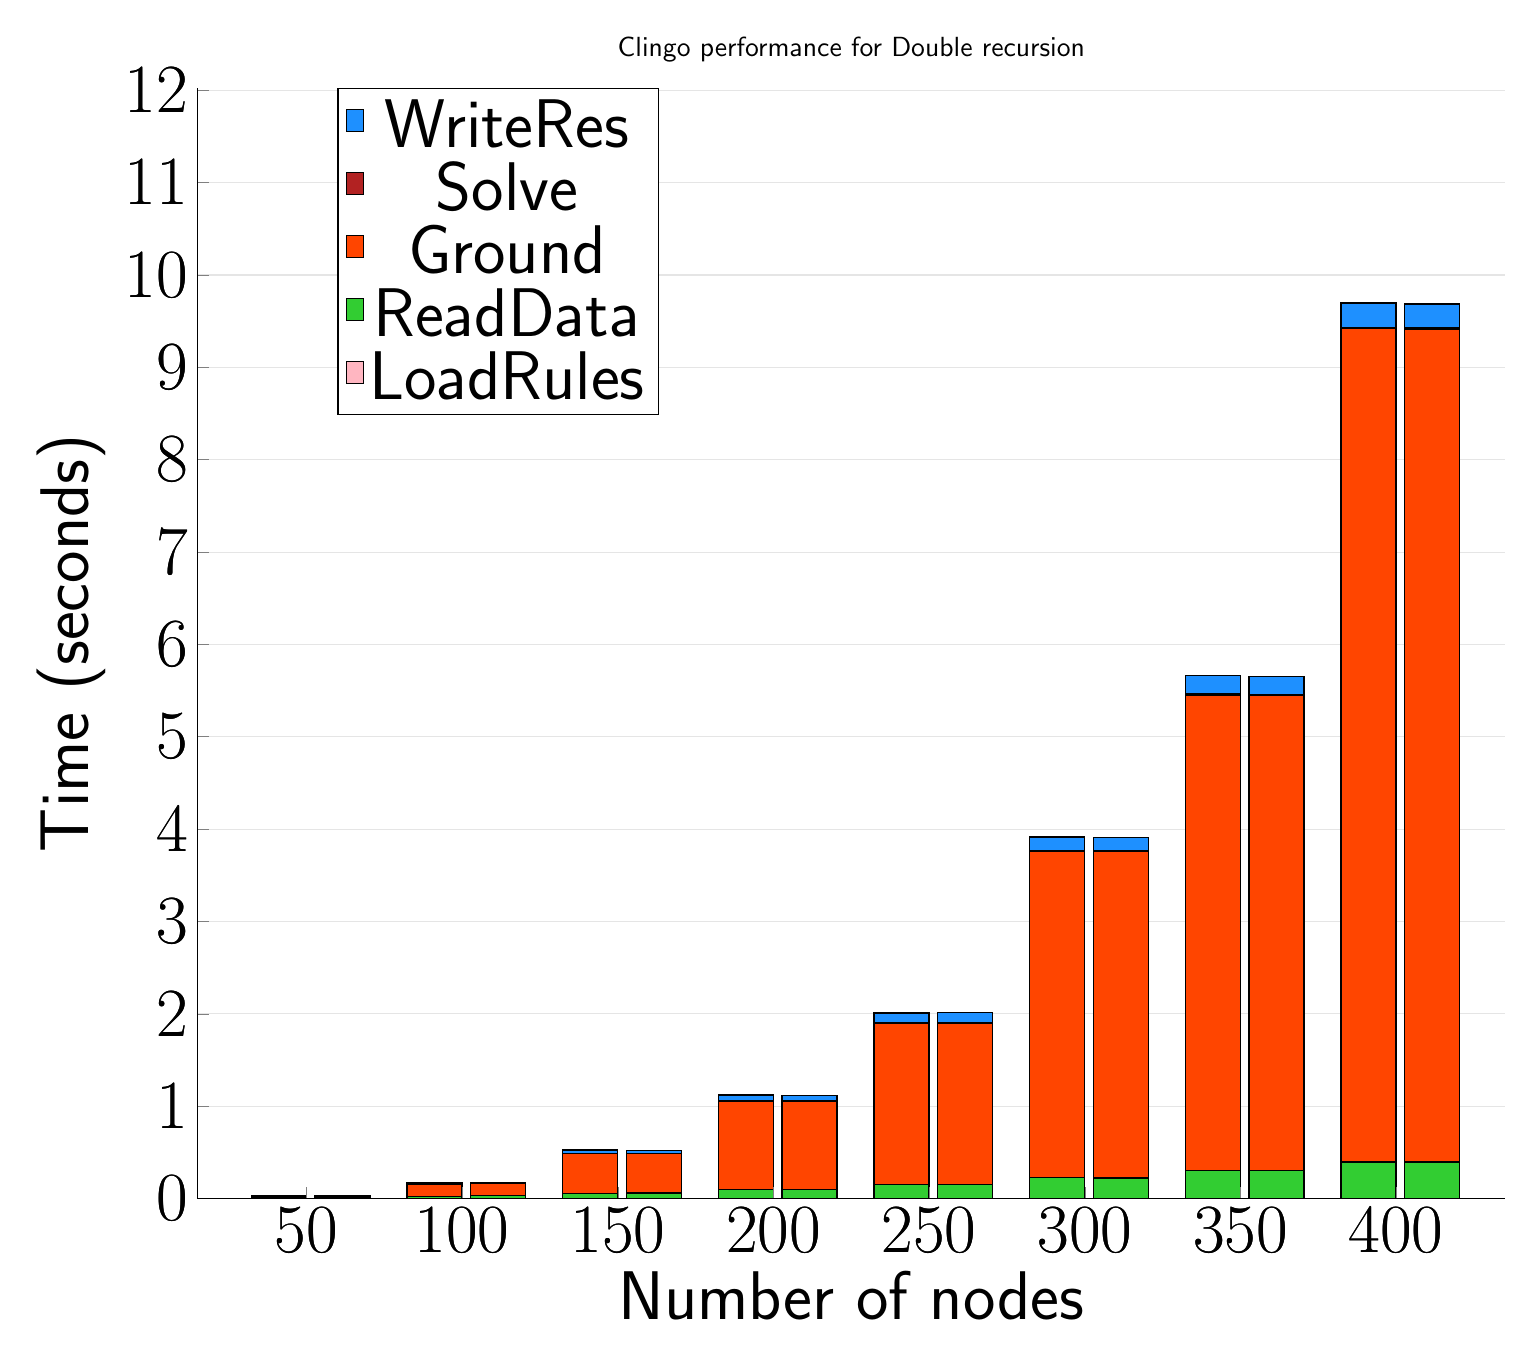
\begin{tikzpicture}
	\begin{axis}[
			ybar stacked,
			title={Clingo performance for Double recursion},
			bar shift=-10pt,
			width=1.5\textwidth,
			bar width=0.7cm,
			ymajorgrids, tick align=inside,
			major grid style={draw=gray!20},
			xtick=data,
			ymin=0, ymax=12.025999999046325,
			axis x line*=bottom,
			axis y line*=left,
			enlarge x limits=0.1,
			legend style={
					at={(0.23, 1)},
					anchor=north,
					legend columns=1,
					font=\Huge,
				},
			ylabel={Time (seconds)},
			xlabel={Number of nodes},
			label style={font=\Huge},
			tick label style={font=\Huge},
		]
		\addlegendimage{fill=DodgerBlue, draw=black, line width=0.2pt}
		\addlegendentry{WriteRes}
		\addlegendimage{fill=FireBrick, draw=black, line width=0.2pt}
		\addlegendentry{Solve}
		\addlegendimage{fill=OrangeRed, draw=black, line width=0.2pt}
		\addlegendentry{Ground}
		\addlegendimage{fill=LimeGreen, draw=black, line width=0.2pt}
		\addlegendentry{ReadData}
		\addlegendimage{fill=LightPink, draw=black, line width=0.2pt}
		\addlegendentry{LoadRules}
		\addplot +[fill=LightPink, draw=black, line width=0.5pt] coordinates {
				(50, 0.0)
				(100, 0.0)
				(150, 0.0)
				(200, 0.0)
				(250, 0.0)
				(300, 0.0)
				(350, 0.0)
				(400, 0.0)
			};
		\addplot +[fill=LimeGreen, draw=black, line width=0.5pt] coordinates {
				(50, 0.005999994277954101)
				(100, 0.025)
				(150, 0.05600001811981201)
				(200, 0.09800000190734863)
				(250, 0.1549999952316284)
				(300, 0.2250000238418579)
				(350, 0.3009999990463257)
				(400, 0.39599993228912356)
			};
		\addplot +[fill=OrangeRed, draw=black, line width=0.5pt] coordinates {
				(50, 0.017999982833862303)
				(100, 0.13100001811981202)
				(150, 0.4329999923706055)
				(200, 0.9559999704360962)
				(250, 1.7480000734329224)
				(300, 3.5370001077651976)
				(350, 5.150999975204468)
				(400, 9.025999999046325)
			};
		\addplot +[fill=FireBrick, draw=black, line width=0.5pt] coordinates {
				(50, 0.0)
				(100, 0.0019999980926513673)
				(150, 0.0019999980926513673)
				(200, 0.004000020027160644)
				(250, 0.004999995231628418)
				(300, 0.008999991416931152)
				(350, 0.009999990463256836)
				(400, 0.012000012397766113)
			};
		\addplot +[fill=DodgerBlue, draw=black, line width=0.5pt] coordinates {
				(50, 0.0039999961853027345)
				(100, 0.014000010490417481)
				(150, 0.03599998950958252)
				(200, 0.06399996280670166)
				(250, 0.10199997425079346)
				(300, 0.14399991035461426)
				(350, 0.19900000095367432)
				(400, 0.2610000133514404)
			};
	\end{axis}
	\begin{axis}[
			ybar stacked,
			bar shift=13pt,
			width=1.5\textwidth,
			bar width=0.7cm,
			ymajorgrids, tick align=inside,
			major grid style={draw=none},
			xtick=data,
			ymin=0, ymax=12.025999999046325,
			axis x line*=none,
			axis y line*=none,
			enlarge x limits=0.1,
			label style={font=\Huge},
			tick label style={font=\Huge},
		]
		\addplot +[fill=LightPink, draw=black, line width=0.5pt] coordinates {
				(50, 0.0)
				(100, 0.0)
				(150, 0.0)
				(200, 0.0)
				(250, 0.0)
				(300, 0.0)
				(350, 0.0)
				(400, 0.0)
			};
		\addplot +[fill=LimeGreen, draw=black, line width=0.5pt] coordinates {
				(50, 0.009999999999999997)
				(100, 0.030000000000000006)
				(150, 0.06000000000000001)
				(200, 0.101)
				(250, 0.152)
				(300, 0.22200000000000003)
				(350, 0.303)
				(400, 0.396)
			};
		\addplot +[fill=OrangeRed, draw=black, line width=0.5pt] coordinates {
				(50, 0.012000000000000002)
				(100, 0.12999999999999998)
				(150, 0.42800000000000005)
				(200, 0.9510000000000002)
				(250, 1.7500000000000004)
				(300, 3.5379999999999994)
				(350, 5.145)
				(400, 9.014999999999999)
			};
		\addplot +[fill=FireBrick, draw=black, line width=0.5pt] coordinates {
				(50, 0.0)
				(100, 0.0)
				(150, 0.0030000000000000027)
				(200, 0.0040000000000000036)
				(250, 0.005000000000000004)
				(300, 0.00799999999999992)
				(350, 0.011999999999999922)
				(400, 0.014999999999999857)
			};
		\addplot +[fill=DodgerBlue, draw=black, line width=0.5pt] coordinates {
				(50, 0.008000000000000002)
				(100, 0.010000000000000009)
				(150, 0.032000000000000015)
				(200, 0.05899999999999983)
				(250, 0.10599999999999996)
				(300, 0.14000000000000018)
				(350, 0.19200000000000012)
				(400, 0.2580000000000003)
			};
	\end{axis}
\end{tikzpicture}

\end{document}
